

Click on the  icon of  \texttt{\getsoftwarename{}} to open the application.
Click the ``SAM" tab to see the configuration of structural analysis model (\Cref{fig:testing}). 
Input the path of OpenSees executable in to ``FEM engine" at the bottom of the SAM tab.



Click ``Analyze" button at the button of the ``Input" panel to start the finite element analysis.
If the application is running correctly, you'll see a progress bar displayed at the middle of the app, which shows the percentage of steps performed. 
When the FE analysis is done, you'll see it shows a message saying ``Analysis is done."  (\Cref{fig:testing}).
And when you click ``I know.", the progress bar will disappear. Now if the ``Play" button is played, you should be able to see animations at the right side of the application.

\begin{figure}[!htbp]
  \centering {
    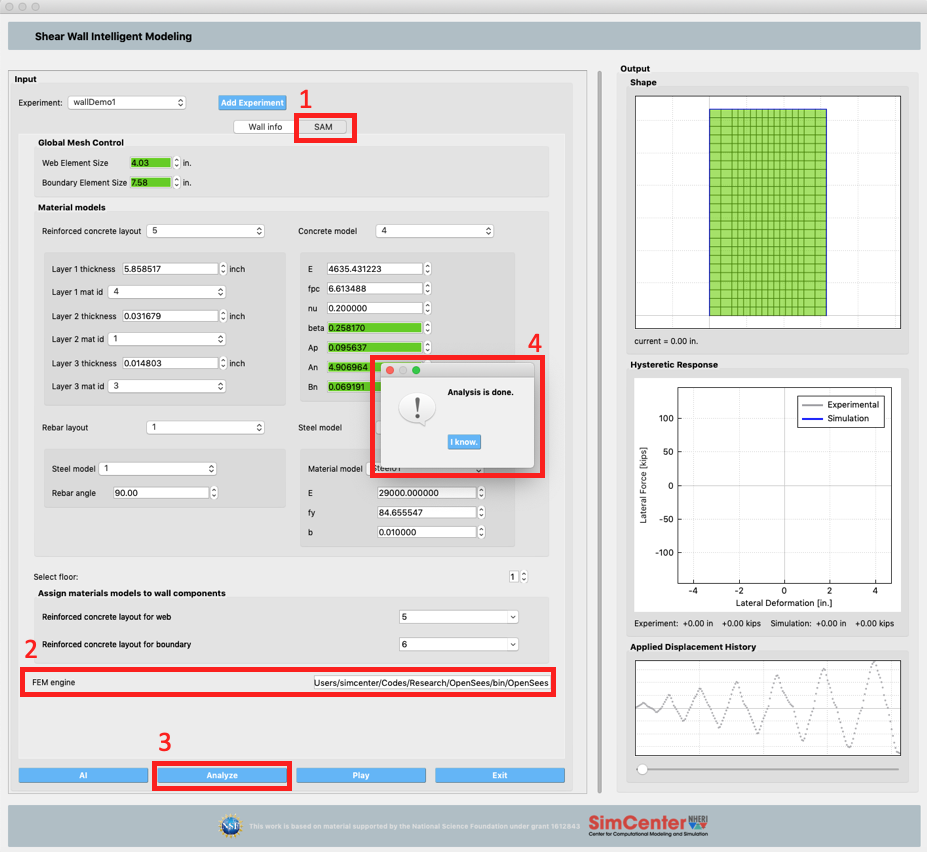
\includegraphics[width=0.6\textwidth]
    {figures/SWIM_analysisisdone-green.png} }
  \caption{Testing SWIM}
  \label{fig:testing}
\end{figure}


